\documentclass[11pt, a4paper]{article}

% Packages
\usepackage[francais]{babel}
\usepackage[T1]{fontenc}
\usepackage[utf8]{inputenc}

\usepackage[left=2cm, right=2cm, top=2cm, bottom=2cm]{geometry}
\usepackage{fancyhdr}
\usepackage{lastpage}
\usepackage{hyperref}

\usepackage{float}

\usepackage{graphicx}
\graphicspath{{./img/}}
\usepackage{tikz}

% Reset paragraph indentation -------------------------------------------------
\setlength{\parindent}{0cm}

% Allow a paragraph to have a linebreak ---------------------------------------
\newcommand{\paragraphnl}[1]{\paragraph{#1}\mbox{}\\}

% Page header and footer ------------------------------------------------------
\pagestyle{fancy}
\setlength{\headheight}{33pt}
\renewcommand{\headrulewidth}{0.5pt}
\lhead{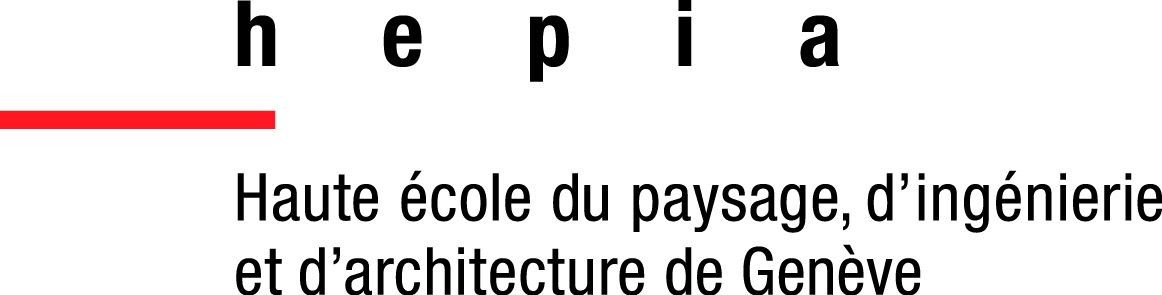
\includegraphics[height=1cm]{hepia.jpg}}
\chead{Jackpot}
\rhead{Claudio Sousa - David Gonzalez}
\renewcommand{\footrulewidth}{0.5pt}
\lfoot{1 février 2017}
\cfoot{}
\rfoot{Page \thepage /\pageref{LastPage}}

% Table of contents depth -----------------------------------------------------
\setcounter{tocdepth}{3}

% Document --------------------------------------------------------------------
\begin{document}

\title
{
    \Huge{Programmation concurrente} \\
    \Huge{Jackpot}
}
\author
{
    \LARGE{David Gonzalez - Claudio Sousa}
}
\date{1 février 2017}
\maketitle

\begin{center}
    %\includegraphics[scale=0.27]{logo.png}
\end{center}

\thispagestyle{empty}

\newpage

% -----------------------------------------------------------------------------
\section{Introduction}

Ce TP de deuxième année consiste à implémenter une machine à sous de Casino multi-tâches.

\subsection{Spécification fonctionnelle}

Chaque partie débute avec l'insertion d'une pièce.
Ensuite, 3 roues tournent à des vitesses différentes.
Chaque roue est arrêtée consécutivement (de gauche à droite)
soit manuellement par l'utilisateur, soit automatiquement après 3 secondes. \\

Lorsque toutes les roues sont arrêtées, le résultat est ajouté à la caisse de la machine.
Ce résultat est calculé selon le nombre de chiffres identiques, les résultats possibles sont:
\begin{itemize}
    \item aucun chiffre identique (perdu);
    \item 2 chiffres identiques (2 pièces gagnées);
    \item 3 chiffres identiques (moitié des pièces en caisse). \\
\end{itemize}

Ce résultat est affiché pendant 5 secondes, puis revient à l'insertion de la pièce.

\subsubsection{Entrées}

Les entrée sont gérées à l'aide de signaux générés par la console avec les touches suivantes:
\begin{itemize}
    \item CTRL-Z (SIGTSTP): insertion d'une pièce;
    \item CTRL-C (SIGINT): arrêt d'une roue manuellement;
    \item CTRL-\textbackslash{} (SIGQUIT): arrêt du jeu.
\end{itemize}

\subsubsection{Threads}

Les threads sont divisés ainsi:
\begin{itemize}
    \item 1 thread pour le controlleur du jeu (qui sera le seul à recevoir les signaux);
    \item 1 thread pour l'affichage;
    \item N threads, 1 pour chaque roue.
\end{itemize}

\newpage

% -----------------------------------------------------------------------------
\section{Development}
\subsection{Architecture}

\begin{figure}[H]
    \begin{center}
        \includegraphics[width=\textwidth]{modules.png}
    \end{center}
    \caption{Architecture du Jackpot}
    \label{Architecture du Jackpot}
\end{figure}

\subsubsection{game\_t et game\_data\_t}
Ces deux structures représentent toutes les données partagées entre les 3 modules pricipaux,
qui sont: \textit{Controller}, \textit{Wheel}, \textit{Display}. \\

La première (\textit{game\_t}) contient les données d'état des roues ainsi que les données de synchronisation. \\

La deuxième (\textit{game\_data\_t}) contient les données du jeu en tant que telle:
la valeur de chaque roue, l'argent restant et l'état final du jeu (gagné, perdu).

\subsubsection{Main}
La fonction principale du programme ne fait que lancer le \textit{Controller}.

\newpage

\subsubsection{Controller}
Ce module est le coeur du programme.
Il est responsable d'instancier le module \textit{Display} ainsi que toutes les instance de \textit{Wheel} (3 par défaut).
Il est également chargé de contrôler l'avancement du jeu selon la machine d'état ci-dessous:

\begin{figure}[H]
    \begin{center}
        \includegraphics[width=0.8\textwidth]{machinestate.png}
    \end{center}
    \caption{Machine d'état du contrôleur}
    \label{Machine d'état du contrôleur}
\end{figure}

\begin{itemize}
    \item \textit{COIN}: état lorsque le jeu est en attente d'une pièce;
    \item \textit{RUN} : état lorsque les roues tournent;
    \item \textit{OVER}: état lorsque le jeu est terminé;
    \item \textit{STOP}: état lorsqu'on quitte le jeu. \\
\end{itemize}

Comme le dit la spécification, les entrée utilisateurs sont gérées par des signaux.
Le \textit{Controller} est donc le seul module (et \textit{thread}) à recevoir et à traiter ces signaux. \\

Les communications sont faitent aux travers des deux structures citées (\textit{game\_t} et \textit{game\_data\_t}),
qu'il est chargé d'instantier et d'initialiser. \\

Au niveau des \textit{threads}, le \textit{Controller} crée lui-même son propre \textit{thread} durant son instanciation.

\subsubsection{Wheel}
Le module \textit{Wheel} est responsable de faire tourner 1 roue (changer le chiffre) dans un \textit{thread} séparé à une certaine fréquence.

\subsubsection{Display}
Le module \textit{Display} a le rôle de gérer l'affichage du jeu dans son \textit{thread}. Donc:
\begin{itemize}
    \item le message de début de parti;
    \item les roues lorsque la parti est en cours;
    \item le résultat de cette parti;
    \item le message lorsqu'on quitte le jeu.
\end{itemize}

\subsubsection{Timer}
Ce module contient deux fonctions utilitaires permettant de mesurer le temps et
d'attendre à une certaine fréquence.

\newpage

% -----------------------------------------------------------------------------
\subsection{Flux d'exécution et synchronisation}
\label{Flux d'exécution et synchronisation}

\begin{figure}[H]
    \begin{center}
        \includegraphics[width=0.95\textwidth]{flow.png}
    \end{center}
    \caption{Flux d'exécution et synchronisation}
    \label{Flux d'exécution et synchronisation}
\end{figure}

\newpage

Le diagramme ci-dessus décrit le flux d'exécution du programme par les différents \textit{threads}.

\subsubsection{Main}
Le \textit{thread} principal commence par lancer le module \textit{Controller}.
Avant de créer son \textit{thread}, le \textit{Controller} bloque tous les signaux
afin que tous les autres \textit{threads} créé après hérite de la configuration. \\
S'ensuit la création du \textit{thread} pour le \textit{Controller}. \\
Le \textit{thread} principal finis sa course par l'attente de la fin du \textit{thread} créé précédement.

\subsubsection{Controller}
Le \textit{Controller} commence par initialiser les structures de données
et lance les modules \textit{Wheel} ainsi que \textit{Display}.
La période d'initialisation se termine par la configuration des signaux à traiter. \\

Ensuite, il rentre dans la boucle du traitement des signaux.
C'est dans celle-ci que la machine d'état (voir figure \ref{Machine d'état du contrôleur}) est configurer.
En effet, 4 signaux différents peuvent être reçus:
\begin{itemize}
    \item SIGTSTP: reinitialise l'état des roues, insert une pièce et configure l'état \textit{RUN};
    \item SIGQUIT: configure le bit de sortie du programme afin que tous les \textit{threads} quittent;
    \item SIGINT ou SIGALRM: met en pause la roue courante,
          si toutes les roue sont en pause, alors l'état \textit{OVER} est configuré. \\
\end{itemize}

Tous les signaux impliquant un changement d'état, tous les \textit{threads}
qui alors attendaient un changement d'états sont réveillés. \\

Finalement, si l'état est \textit{OVER} en fin de boucle, alors le \textit{Controller} calcule le résultat du jeu,
attends les 5 secondes pour l'affichage de celui-ci, configure l'état \textit{COIN} et réveille à nouveau les \textit{threads}. \\

La boucle continue indéfiniment tant que le bit de sorti n'est pas configuré.

\subsubsection{Wheel}
Lors du lancement d'une roue, le \textit{thread} du \textit{Controller} commence par créer le \textit{thread} de cette roue
en lui passant en paramètre la structure de synchronisation ainsi que le chiffre que la roue va traiter.
Le \textit{thread} nouvellement créé rentre immédiatement dans sa boucle qui s'exécute comme suit: \\

Il commence par vérifier qu'il n'est pas en pause. Si oui, alors il se met en attente jusqu'au prochain changement d'état.
Dans les deux cas, il continue sa route en mettant à jour la valeur de la roue puis attends sa fréquence de rafraichissement. \\

Le flux ci-dessus s'exécute indéfiniment tant que la bit de sorti n'est pas configuré.

\subsubsection{Display}
Lorsque  le \textit{thread} du \textit{Controller} initialise le module \textit{Display},
un \textit{thread} est créé pour lui. Sa boucle d'exécution est basé sur la machine d'état:
\begin{itemize}
    \item \textit{COIN}: simplement affiche le message et attends le changement d'état;
    \item \textit{RUN}: tant que cet état est actif, affiche les roues et attends sa fréquence de rafraichissement.
                        lorsque le jeu passe en état \textit{OVER}, affiche le résultat et attends l'état suivant. \\
\end{itemize}

Comme pour les autres, la boucle ne se termine pas tant que la bit de sorti n'est pas configuré.

\newpage

% -----------------------------------------------------------------------------
\subsection{Méthodologie de travail}
\subsubsection{Répartition du travail}

Ce travail a été effectué à deux.

Nous avons commencés par réfléchir sur papier sur deux éléments:

\begin{itemize}
    \item architecture du programme: modules et interfaces de bases;
    \item flux d'exécution général du programme. \\
\end{itemize}

Ensuite, le travail a été réparti ainsi:
\begin{itemize}
    \item ... \\
\end{itemize}

Finalement, nous avons mis en commun les modules et finalisés la synchronisation des threads des différents modules.

\newpage

\end{document}
